\documentclass[11pt]{article}
\usepackage{graphicx}
\usepackage{lineno, blindtext}
\usepackage{setspace}
\usepackage{comment}

\linenumbers
\setstretch{1.5} %spacing with setspace
\setlength{\topmargin}{-2cm}
\setlength{\oddsidemargin}{0cm}
\setlength{\textheight}{24cm}
\setlength{\textwidth}{16cm}

\title{A punny title \\ \large A less punny subtitle \\} %here we add the subtitle as well

\author{Amisha Bhojwani}

\date{1st December, 2020}

\begin{document}
  
  \begin{titlepage}
    \maketitle
  \end{titlepage}
  
  \tableofcontents{}
  \pagebreak

  \section{Introduction}
  \begin{itemize}
    \item[--] Explain what a functional response is 
    \item[--] How do we analyse a functional response? Explain the phenomenological approach
    \item[--] Explain the types of functional response. A brief timeline of functional response models, variables and ecological theory considered. 
    \item[--] Explain the limitations of each type according to foraging theory, including the consideration that the Holling disc equation
    should be considered phenomenological rather than mechanistic (cite Jeschke 2002) - maybe this should go in discussion
    \item[--] Introduce the dataset: whats recorded and for what main taxons
    \item[--] Ask the study question
  \end{itemize}

  \section{Methods}
    \subsection{Computing tools}
      \begin{itemize}
        \item[--] Used R for model fitting and plotting. Wrangling and data visualisation seems more comfortable for me in R. I am more familiar
        with the commands and syntax, it is more logical to me than using Python. I like working with matrices in R because they are easily
        manipulatable, don't have a grasp on objects in Python yet, although it would have been interesting to have written model fitting in
        python simply to make the scripts easily importable modules in a final model compiling script.
        \item[--] Used Python to write a compiling script. Will use subprocess module in Python to run the different stages of model fitting.
        \item[--] Used Latex to compile report (because Samraat said so)
      \end{itemize}
        
    \subsection{Model fitting}
      \begin{itemize}
        \item[--] Models chosen: quadratic linear, cubic linear - achieved, need polishing for figures. Want to pursue Holling Type II but starting
        values obtained from sampling are devoid of biological meaning. Must be an error in syntax that i cant spot. For some subsets it looks ok when using sampling and bounding.
        \item[--] If Holling II achieved: explain parameter estimating and sampling/reasoning behind bounding
        \item[--] Explain parameters chosen to compare fits: R2, AIC, BIC . Still need to consider AICc and other options.
      \end{itemize}

  \section{Results}
    \begin{itemize}
        \item[--] Summary table showing statistics of various fits
        \item[--] Example figure of how quadratic and cubic linear models fit on a subset of the data:
            \begin{figure}[h]
                \centering
                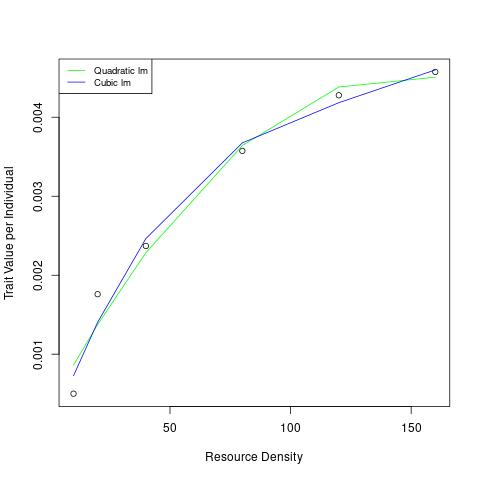
\includegraphics[scale=0.5]{subset_39882_plot.jpeg}  
                \caption{A very polishable figure. Working on smooth and clean versions on ggplot. This one is jpeg but submission ones will be pdf.}
            \end{figure}
    \end{itemize}

  \section{Discussion}

  \section{Conclusion}

  \section{Bibliography}
  \begin{itemize}
    \item[--] So far i have gone through the core readings. I'm reading the paper Alex posted where he got samples for fitting Holling type III (Rosenbaum 2018)
  \end{itemize}
\end{document}